% Generated by pysimcount.pftcount -- do not edit; regenerate instead.
% figure: tcount-vs-n -- T-count vs n, Suzuki (dashed) vs optimised (solid), colour = order
% metric=t gatebase=ct merged; mean over seeds [1, 2, 3, 4, 5, 6, 7, 8, 9, 10], bars = min..max; measured r (filled); open markers: r from each seed's power-law fit on n = [6, 7, 8, 10], circuit synthesised at that r (extrapolated)
% formulas: Suzuki S4, M&O q=6 (rec., Tab. 2), Suzuki S6, M&O q=14 (rec., Tab. 3), Blanes & Moan q=10, Suzuki S8, Morales m=8 (17 steps)
% figure made at git_commit=e42ff29056ad9ea7fc7c9899fab334903e42e3e3 git_dirty=True
% derived: tcount-vs-n.tex restyled by pysimcount.figuniform: extrapolated points (r from power-law fit) drawn in their series' measured style, style-key legend entries removed; extrapolated n = [13, 20]; source_sha256=c39b229024f3185b7dea8bbc46e7a204e9037e05dd5770b17104f32bc3a6ecdb
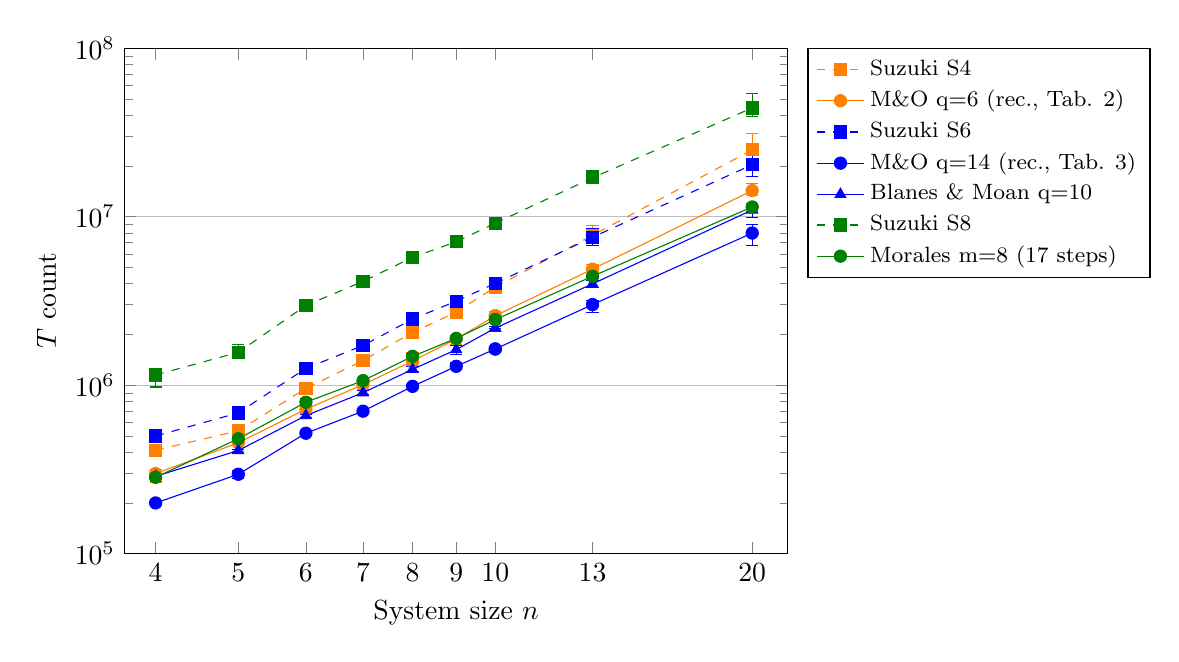
\begin{tikzpicture}
  \begin{loglogaxis}[
    width=10cm, height=8cm,
    xlabel={System size $n$}, ylabel={$T$ count},
    xmin=3.68, xmax=22, ymin=100000, ymax=1e+08,
    xtick={4,5,6,7,8,9,10,13,20}, xticklabels={4,5,6,7,8,9,10,13,20},
    ymajorgrids=true, legend pos=outer north east, legend cell align=left,
    legend style={font=\footnotesize},
  ]
    \addplot[orange, dashed, mark=square*, mark size=2.2pt, mark options={solid, fill=orange}, error bars/.cd, y dir=both, y explicit, error bar style={orange, solid}] coordinates {
      (4,410227) += (0,4385) -= (0,12011)
      (5,535141) += (0,32099) -= (0,18901)
      (6,956087) += (0,61533) -= (0,60737)
      (7,1398590) += (0,65506) -= (0,81150)
      (8,2052152) += (0,77768) -= (0,99724)
      (9,2712542) += (0,149152) -= (0,153838)
      (10,3814178) += (0,343128) -= (0,119398)
    };
    \addlegendentry{Suzuki S4}
    \addplot[orange, dashed, mark=square*, mark size=2.2pt, mark options={solid, fill=orange}, forget plot, error bars/.cd, y dir=both, y explicit, error bar style={orange, solid}] coordinates {
      (10,3814178) += (0,0) -= (0,0)
      (13,7745687) += (0,1066069) -= (0,617671)
      (20,24911670) += (0,6248004) -= (0,3635184)
    };
    \addplot[orange, solid, mark=*, mark size=2.2pt, mark options={solid, fill=orange}, error bars/.cd, y dir=both, y explicit, error bar style={orange, solid}] coordinates {
      (4,298204) += (0,16516) -= (0,33724)
      (5,454337) += (0,24967) -= (0,48761)
      (6,719342) += (0,24990) -= (0,41182)
      (7,1005067) += (0,53081) -= (0,64379)
      (8,1389715) += (0,165321) -= (0,79491)
      (9,1875411) += (0,104483) -= (0,135387)
      (10,2579888) += (0,145168) -= (0,180656)
    };
    \addlegendentry{M\&O q=6 (rec., Tab. 2)}
    \addplot[orange, solid, mark=*, mark size=2.2pt, mark options={solid, fill=orange}, forget plot, error bars/.cd, y dir=both, y explicit, error bar style={orange, solid}] coordinates {
      (10,2579888) += (0,0) -= (0,0)
      (13,4878507) += (0,343633) -= (0,199489)
      (20,14282311) += (0,1418885) -= (0,879247)
    };
    \addplot[blue, dashed, mark=square*, mark size=2.2pt, mark options={solid, fill=blue}, error bars/.cd, y dir=both, y explicit, error bar style={blue, solid}] coordinates {
      (4,498655) += (0,32701) -= (0,9101)
      (5,683636) += (0,27514) -= (0,12392)
      (6,1257090) += (0,61766) -= (0,83890)
      (7,1716813) += (0,84051) -= (0,117761)
      (8,2463415) += (0,76167) -= (0,20335)
      (9,3147913) += (0,160987) -= (0,93103)
      (10,4012921) += (0,303067) -= (0,211911)
    };
    \addlegendentry{Suzuki S6}
    \addplot[blue, dashed, mark=square*, mark size=2.2pt, mark options={solid, fill=blue}, forget plot, error bars/.cd, y dir=both, y explicit, error bar style={blue, solid}] coordinates {
      (10,4012921) += (0,0) -= (0,0)
      (13,7544299) += (0,944741) -= (0,830907)
      (20,20321667) += (0,4353971) -= (0,2975715)
    };
    \addplot[blue, solid, mark=*, mark size=2.2pt, mark options={solid, fill=blue}, error bars/.cd, y dir=both, y explicit, error bar style={blue, solid}] coordinates {
      (4,199644) += (0,156) -= (0,284)
      (5,295456) += (0,15464) -= (0,15704)
      (6,517803) += (0,21981) -= (0,9899)
      (7,700110) += (0,16304) -= (0,25074)
      (8,982626) += (0,25418) -= (0,17002)
      (9,1292116) += (0,59288) -= (0,40566)
      (10,1637724) += (0,50796) -= (0,66588)
    };
    \addlegendentry{M\&O q=14 (rec., Tab. 3)}
    \addplot[blue, solid, mark=*, mark size=2.2pt, mark options={solid, fill=blue}, forget plot, error bars/.cd, y dir=both, y explicit, error bar style={blue, solid}] coordinates {
      (10,1637724) += (0,0) -= (0,0)
      (13,3004156) += (0,170792) -= (0,300988)
      (20,7987145) += (0,959735) -= (0,1258633)
    };
    \addplot[blue, solid, mark=triangle*, mark size=2.2pt, mark options={solid, fill=blue}, error bars/.cd, y dir=both, y explicit, error bar style={blue, solid}] coordinates {
      (4,287233) += (0,5967) -= (0,8617)
      (5,408923) += (0,4589) -= (0,16769)
      (6,658784) += (0,7868) -= (0,17360)
      (7,901238) += (0,22542) -= (0,24694)
      (8,1239448) += (0,56480) -= (0,33632)
      (9,1624357) += (0,90391) -= (0,104629)
      (10,2178800) += (0,37144) -= (0,61776)
    };
    \addlegendentry{Blanes \& Moan q=10}
    \addplot[blue, solid, mark=triangle*, mark size=2.2pt, mark options={solid, fill=blue}, forget plot, error bars/.cd, y dir=both, y explicit, error bar style={blue, solid}] coordinates {
      (10,2178800) += (0,0) -= (0,0)
      (13,3990068) += (0,168532) -= (0,216320)
      (20,10946177) += (0,835087) -= (0,1087489)
    };
    \addplot[green!50!black, dashed, mark=square*, mark size=2.2pt, mark options={solid, fill=green!50!black}, error bars/.cd, y dir=both, y explicit, error bar style={green!50!black, solid}] coordinates {
      (4,1147832) += (0,22468) -= (0,173312)
      (5,1564733) += (0,186625) -= (0,81665)
      (6,2967788) += (0,98492) -= (0,225578)
      (7,4126735) += (0,257393) -= (0,118225)
      (8,5725360) += (0,217276) -= (0,217234)
      (9,7091892) += (0,76848) -= (0,286240)
      (10,9141777) += (0,522855) -= (0,68741)
    };
    \addlegendentry{Suzuki S8}
    \addplot[green!50!black, dashed, mark=square*, mark size=2.2pt, mark options={solid, fill=green!50!black}, forget plot, error bars/.cd, y dir=both, y explicit, error bar style={green!50!black, solid}] coordinates {
      (10,9141777) += (0,0) -= (0,0)
      (13,16991266) += (0,1772726) -= (0,1050594)
      (20,44173940) += (0,9729228) -= (0,4752300)
    };
    \addplot[green!50!black, solid, mark=*, mark size=2.2pt, mark options={solid, fill=green!50!black}, error bars/.cd, y dir=both, y explicit, error bar style={green!50!black, solid}] coordinates {
      (4,283483) += (0,15077) -= (0,14775)
      (5,480273) += (0,27567) -= (0,4293)
      (6,790926) += (0,38574) -= (0,5206)
      (7,1062267) += (0,12523) -= (0,45515)
      (8,1480735) += (0,49073) -= (0,12907)
      (9,1892882) += (0,79598) -= (0,47402)
      (10,2446100) += (0,66196) -= (0,18780)
    };
    \addlegendentry{Morales m=8 (17 steps)}
    \addplot[green!50!black, solid, mark=*, mark size=2.2pt, mark options={solid, fill=green!50!black}, forget plot, error bars/.cd, y dir=both, y explicit, error bar style={green!50!black, solid}] coordinates {
      (10,2446100) += (0,0) -= (0,0)
      (13,4424857) += (0,127929) -= (0,121557)
      (20,11407316) += (0,599884) -= (0,709888)
    };
  \end{loglogaxis}
\end{tikzpicture}
